\documentclass[10pt,a4paper,twoside,extrafontsizes]{memoir}
\usepackage{amsmath,amssymb,amsfonts} % Typical maths resource packages
\usepackage{graphics}                 % Packages to allow inclusion of graphics
\usepackage{color}                    % For creating coloured text and background
\usepackage[plainpages=false,pdfpagelabels]{hyperref}                 % For creating hyperlinks in cross references
\usepackage{listings}
\usepackage{dirtree}

\hyphenation{OpenIMAJ}

%config code listings
\lstset{ %
breaklines=true,                % sets automatic line breaking
basicstyle=\ttfamily,
showspaces=false,
showtabs=false
}

%config formatting
\setlength{\parindent}{0pt}
\setlength{\parskip}{1ex plus 0.5ex minus 0.2ex}

\settrimmedsize{297mm}{210mm}{*}
\setlength{\trimtop}{0pt}
\setlength{\trimedge}{0pt}
\settypeblocksize{634pt}{348.13pt}{*}
\setulmargins{4cm}{*}{*}
\setlrmargins{3cm}{*}{1.5}
\setmarginnotes{17pt}{91pt}{\onelineskip}
\setheadfoot{\onelineskip}{2\onelineskip}
\setheaderspaces{*}{2\onelineskip}{*}
\checkandfixthelayout

\newlength\titlepage
\setlength{\titlepage}{\paperwidth}
\addtolength{\titlepage}{-\spinemargin}
\addtolength{\titlepage}{-1.5cm}

\newlength\titlepagefull
\setlength{\titlepagefull}{\paperwidth}
\addtolength{\titlepagefull}{-\spinemargin}

%config chapter headings
\usepackage{color,calc,graphicx,soul,fourier}
\definecolor{nicered}{rgb}{.647,.129,.149}
\makeatletter
\newlength\dlf@normtxtw
\setlength\dlf@normtxtw{\textwidth}
\def\myhelvetfont{\def\sfdefault{mdput}}
\newsavebox{\feline@chapter}
\newcommand\feline@chapter@marker[1][4cm]{%
  \sbox\feline@chapter{%
    \resizebox{!}{#1}{\fboxsep=1pt%
      \colorbox{nicered}{\color{white}\bfseries\sffamily\thechapter}%
    }}%
  \rotatebox{90}{%
    \resizebox{%
      \heightof{\usebox{\feline@chapter}}+\depthof{\usebox{\feline@chapter}}}%
     {!}{\scshape\so\@chapapp}}\quad%
  \raisebox{\depthof{\usebox{\feline@chapter}}}{\usebox{\feline@chapter}}%
}
\newcommand\feline@chm[1][4cm]{%
  \sbox\feline@chapter{\feline@chapter@marker[#1]}%
  \makebox[0pt][l]{% aka \rlap
    \makebox[1cm][r]{\usebox\feline@chapter}%
  }}
\makechapterstyle{daleif1}{
  \renewcommand\chapnamefont{\normalfont\Large\scshape\raggedleft\so}
  \renewcommand\chaptitlefont{\normalfont\huge\bfseries\scshape\color{nicered}}
  \renewcommand\chapternamenum{}
  \renewcommand\printchaptername{}
  \renewcommand\printchapternum{\null\hfill\feline@chm[2.5cm]\par}
  \renewcommand\afterchapternum{\par\vskip\midchapskip}
  \renewcommand\printchaptertitle[1]{\chaptitlefont\raggedleft ##1\par}
}
\makeatother
\chapterstyle{daleif1}

\renewcommand{\chaptername}{Tutorial}%

\makeindex

\begin{document}	
% \maketitle
\pagestyle{empty}
\pagenumbering{alph}
 %%% Title, author, publisher, etc.,  here

\begin{minipage}{0.5\titlepage}

\includegraphics{OpenIMAJ.png}
\end{minipage}
\hspace{0.001pt}
\begin{minipage}{0.5\titlepage}
\Huge
\flushright
Jonathon Hare\\
Sina Samangooei\\
David Dupplaw
\end{minipage}
\\[10cm]
\begin{minipage}{\titlepage}
\fontsize{60}{100}\selectfont\flushright The
\end{minipage}
\\[1cm]
\colorbox{nicered}{\parbox{\titlepagefull}{
	\parbox{\titlepage}{
		\color{white}\fontsize{80}{120}\selectfont\flushright OpenIMAJ\\[0.4cm]}
	}
}
\\[0.8cm]
\begin{minipage}{\titlepage}
\fontsize{60}{100}\selectfont\flushright Tutorial
\end{minipage}
%\cleardoublepage
\clearpage
\textbf{{\LARGE Jonathon Hare,} Ph.D.}\\
Electronics and Computer Science\\
The University of Southampton\\
\url{http://www.ecs.soton.ac.uk/~jsh2}\\[0.5cm]
\textbf{{\LARGE Sina Samangooei,} Ph.D.}\\
Electronics and Computer Science\\
The University of Southampton\\
\url{http://www.ecs.soton.ac.uk/~ss}\\[0.5cm]
\textbf{{\LARGE David Dupplaw,} Ph.D.}\\
Electronics and Computer Science\\
The University of Southampton\\
\url{http://www.ecs.soton.ac.uk/~dpd}
\\[2cm]
Copyright \copyright 2011 The University of Southampton and the individual authors.\\[0.5cm]

\begin{figure}[h!]
\center

\includegraphics[width=0.5\textwidth]{cc-logo.eps}\\[0.5cm]
\end{figure}

The OpenIMAJ Tutorial is licensed under a Creative Commons Attribution-ShareAlike 3.0 Unported License. To view a copy of this license visit:\\
\url{http://creativecommons.org/licenses/by-sa/3.0/legalcode}
\\[0.5cm]

\begin{figure}[h!]
\center
\includegraphics[width=0.5\textwidth]{by-sa.eps}
\end{figure}

\begin{figure}[b!]
\begin{minipage}{\textwidth}
Current development of the OpenIMAJ and ImageTerrier software is funded by the European Union Seventh Framework Programme (FP7/2007-2013) under grant agreement n$^{\circ}$ 270239 (ARCOMEM) and 231126 (LivingKnowledge) together with the LiveMemories project, graciously funded by the Autonomous Province of Trento (Italy). We are also grateful to the Arts and Humanities Research Council (`Bridging the Semantic Gap' - MRG-AN6770/APN17429) and Ordnance Survey, for earlier funding under which a number of the older OpenIMAJ classes were created.
\end{minipage}
\end{figure}
\cleardoublepage
\pagenumbering{roman}
\tableofcontents*

\chapter*{Preface}\normalsize
\addcontentsline{toc}{chapter}{Preface}
\pagestyle{plain}

\textbf{OpenIMAJ} is a set of libraries and tools for multimedia analysis. 
OpenIMAJ is very broad and contains everything from state-of-the-art computer 
vision (e.g. SIFT descriptors, salient region detection, face detection, etc.) 
and advanced data clustering, through to software that performs analysis on the 
layout and structure of webpages.

OpenIMAJ is primarily written in pure Java and, as such, is completely platform 
independent. The video capture and hardware libraries contain some native code 
but Linux (x86 and x86\_64 are supported currently; ARM support is coming soon), 
OSX and Windows are supported out of the box (under both 32 and 64 bit JVMs). 
It is possible to write programs that use the libraries in any JVM language 
that supports Java interoperability, such as Groovy, Jython, JRuby or 
Scala. OpenIMAJ can even be run on Android phones and tablets.

The OpenIMAJ software is structured into a number of modules. The modules 
can be used independently, so if, for instance, you were developing data 
clustering software using OpenIMAJ you wouldn't need to acquire the modules related 
to images. The list on the following page illustrates the modules 
and summarises the functionality in each component.

This tutorial aims to instruct the reader on how to get up and running
writing code using OpenIMAJ. Currently the tutorial covers the following areas:
\begin{enumerate}
	\item Getting started with OpenIMAJ using Maven
	\item Processing your first image
	\item Introduction to clustering, segmentation and connected components
	\item Processing video
	\item Finding faces
	\item Global image features
	\item SIFT and feature matching
\end{enumerate}

In the future we hope to add more content to the tutorial covering the following:
\begin{itemize}
	\item Image and video indexing using ImageTerrier
	\item Compiling OpenIMAJ from source
	\item Tracking features in video
	\item Audio processing
	\item Hardware interfaces
	\item Advanced local features
	\item Scalable processing with OpenIMAJ/Hadoop
	\item Machine learning
\end{itemize}

\section*{The OpenIMAJ Modules}

\begin{figure*}[h!]
\renewcommand*\DTstylecomment{\rmfamily{ }{ }}
\newcommand{\descwidth}{8.0cm} 
\DTsetlength{0.2em}{0.4em}{0.2em}{0.4pt}{1.6pt}
\dirtree{%
.1 openimaj.
.2 core \DTcomment{\begin{minipage}[t]{\descwidth}
Submodule for modules containing functionality used across the library.
\end{minipage}}.
.3 core \DTcomment{\begin{minipage}[t]{\descwidth}
Core library functionality concerned with general programming problems rather than multimedia specific functionality. Includes I/O utilities, randomisation, hashing and type conversion.
\end{minipage}}.
.3 feature \DTcomment{\begin{minipage}[t]{\descwidth}
Core notion of features, usually denoted as arrays of data. Definitions of features for all primitive types, features with location and lists of features (both in memory and on disk).
\end{minipage}}.
.3 audio \DTcomment{\begin{minipage}[t]{\descwidth}
Core definitions of audio streams and samples/chunks. Also contains interfaces for processors for these basic types.
\end{minipage}}.
.3 image \DTcomment{\begin{minipage}[t]{\descwidth}
Core definitions of images, pixels and connected components. Also contains interfaces for processors for these basic types.
\end{minipage}}.
.3 video \DTcomment{\begin{minipage}[t]{\descwidth}
Core definitions of a video type and functionality for displaying and processing videos.
\end{minipage}}.
.3 video-capture \DTcomment{\begin{minipage}[t]{\descwidth}
Cross-platform video capture interface using a lightweight native interface. Supports 32 and 64 bit JVMs under Linux, OSX and Windows.
\end{minipage}}.
.3 math \DTcomment{\begin{minipage}[t]{\descwidth}
Mathematical implementations including geometric, matrix and statistical operators. 
\end{minipage}}.
.2 audio \DTcomment{\begin{minipage}[t]{\descwidth}
Submodule for audio related functionality.
\end{minipage}}.
.3 processing \DTcomment{\begin{minipage}[t]{\descwidth}
Implementations of various audio processors (e.g. multichannel conversion, volume change, ...).
\end{minipage}}.
.2 ....
}
\end{figure*}

\begin{figure*}[h!]
\renewcommand*\DTstylecomment{\rmfamily{ }{ }}
\newcommand{\descwidth}{8.0cm} 
\DTsetlength{0.2em}{0.4em}{0.2em}{0.4pt}{1.6pt}
\dirtree{%
.1 ....
.2 image \DTcomment{\begin{minipage}[t]{\descwidth}
Submodule for image related functionality.
\end{minipage}}.
.3 processing \DTcomment{\begin{minipage}[t]{\descwidth}
Implementations of various image, pixel and connected component processors (resizing, convolution, edge detection, ...).
\end{minipage}}.
.3 feature-extraction \DTcomment{\begin{minipage}[t]{\descwidth}
Methods for the extraction of low-level image features, including global image features and pixel/patch classification models.
\end{minipage}}.
.3 local-features \DTcomment{\begin{minipage}[t]{\descwidth}
Methods for the extraction of local features. Local features are descriptions of regions of images (SIFT, ...) selected by detectors (Difference of Gaussian, Harris, ...). 
\end{minipage}}.
.3 faces \DTcomment{\begin{minipage}[t]{\descwidth}
Implementation of a flexible face-recognition pipeline, including pluggable detectors, aligners, feature extractors and recognisers.
\end{minipage}}.
.2 machine-learning \DTcomment{\begin{minipage}[t]{\descwidth}
Algorithms which aid the classification and search of data.
\end{minipage}}.
.3 nearest-neighbour \DTcomment{\begin{minipage}[t]{\descwidth}
Brute force and KD-Tree implementations of exact and approximate KNN.
\end{minipage}}.
.3 clustering \DTcomment{\begin{minipage}[t]{\descwidth}
Various clustering algorithm implementations for all primitive types including random, random forest, \mbox{K-Means} (Exact, Hierarchical and Approximate), ...
\end{minipage}}.
.2 hadoop \DTcomment{\begin{minipage}[t]{\descwidth}
Extensions to enable interaction with the Apache Hadoop Map-Reduce implementation.
\end{minipage}}.
.3 core-hadoop \DTcomment{\begin{minipage}[t]{\descwidth}
Reusable wrappers to access and create sequence-files and map-reduce jobs.
\end{minipage}}.
.3 tools \DTcomment{\begin{minipage}[t]{\descwidth}
Tools that provide Map-Reduce jobs that can be run on a Hadoop cluster.
\end{minipage}}.
.4 HadoopClusterQuantiserTool \DTcomment{\begin{minipage}[t]{\descwidth}
Distributed feature quantisation tool.
\end{minipage}}.
.4 HadoopFastKMeans \DTcomment{\begin{minipage}[t]{\descwidth}
Distributed feature clustering tool.
\end{minipage}}.
.4 HadoopGlobalFeaturesTool \DTcomment{\begin{minipage}[t]{\descwidth}
Distributed global image feature extraction tool.
\end{minipage}}.
.4 HadoopImageDownload \DTcomment{\begin{minipage}[t]{\descwidth}
Distributed image download tool.
\end{minipage}}.
.4 HadoopLocalFeaturesTool \DTcomment{\begin{minipage}[t]{\descwidth}
Distributed local image feature extraction tool.
\end{minipage}}.
.4 SequenceFileIndexer \DTcomment{\begin{minipage}[t]{\descwidth}
Tool for building an index of the keys in a Hadoop SequenceFile.
\end{minipage}}.
.4 SequenceFileTool \DTcomment{\begin{minipage}[t]{\descwidth}
Tool for building, inspecting and extracting Hadoop SequenceFiles.
\end{minipage}}.
.2 hardware \DTcomment{\begin{minipage}[t]{\descwidth}
Various interfaces to hardware devices that we've used in projects built using OpenIMAJ.
\end{minipage}}.
.3 serial \DTcomment{\begin{minipage}[t]{\descwidth}
Interface to hardware devices that connect to serial or USB-serial ports.
\end{minipage}}.
.3 gps \DTcomment{\begin{minipage}[t]{\descwidth}
Interface to GPS devices that support the NMEA protocol.
\end{minipage}}.
.3 compass \DTcomment{\begin{minipage}[t]{\descwidth}
Interface to an OceanServer OS5000 digital compass.
\end{minipage}}.
.2 ....
}
\end{figure*}

\begin{figure*}[h!]
\renewcommand*\DTstylecomment{\rmfamily{ }{ }}
\newcommand{\descwidth}{8.0cm} 
\DTsetlength{0.2em}{0.4em}{0.2em}{0.4pt}{1.6pt}
\dirtree{%
.1 ....
.2 web \DTcomment{\begin{minipage}[t]{\descwidth}
Support for analysing and processing web-pages.
\end{minipage}}.
.3 core-web \DTcomment{\begin{minipage}[t]{\descwidth}
Implementation of a programatic offscreen web browser and utility functions.
\end{minipage}}.
.3 analysis \DTcomment{\begin{minipage}[t]{\descwidth}
Utilities for analysing the content and visual layout of a web-page.
\end{minipage}}.
.2 video \DTcomment{\begin{minipage}[t]{\descwidth}
Support for analysing and processing video.
\end{minipage}}.
.3 video-processing \DTcomment{\begin{minipage}[t]{\descwidth}
Various video processing algorithms, such as shot-boundary detection.
\end{minipage}}.
.3 xuggle-video \DTcomment{\begin{minipage}[t]{\descwidth}
Plugin to use Xuggler as a video source. Allows most video formats to be read into OpenIMAJ.
\end{minipage}}.
.2 thirdparty \DTcomment{\begin{minipage}[t]{\descwidth}
Thirdparty code that has been integrated into OpenIMAJ.
\end{minipage}}.
.3 klt-tracker \DTcomment{\begin{minipage}[t]{\descwidth}
Implementation of the Kanade-Lucus-Tomasi feature tracker.
\end{minipage}}.
.2 tools \DTcomment{\begin{minipage}[t]{\descwidth}
Commandline tools exposing OpenIMAJ functionality
\end{minipage}}.
.3 CityLandscapeClassifier \DTcomment{\begin{minipage}[t]{\descwidth}
Tool for classifying images as being cityscapes/landscapes (or natural/unnatural).
\end{minipage}}.
.3 FaceTools \DTcomment{\begin{minipage}[t]{\descwidth}
Tools for face detection and recognition.
\end{minipage}}.
.3 FeatureVisualisation \DTcomment{\begin{minipage}[t]{\descwidth}
Tools for visualising certain types of image feature.
\end{minipage}}.
.3 FlickrCrawler \DTcomment{\begin{minipage}[t]{\descwidth}
Tool for downloading image datasets from Flickr.
\end{minipage}}.
.3 GlobalFeaturesTool \DTcomment{\begin{minipage}[t]{\descwidth}
Tool for extracting global features from images.
\end{minipage}}.
.3 ImageCollectionTool \DTcomment{\begin{minipage}[t]{\descwidth}
Tool for creating collections of images from various sources.
\end{minipage}}.
.3 LocalFeaturesTool \DTcomment{\begin{minipage}[t]{\descwidth}
Tool for extracting local features from images.
\end{minipage}}.
.3 OCRTools \DTcomment{\begin{minipage}[t]{\descwidth}
Tool for applying OCR to images.
\end{minipage}}.
.3 WebTools \DTcomment{\begin{minipage}[t]{\descwidth}
Tools for extracting and analysing the layout and visual characteristics of webpages.
\end{minipage}}.
}
\end{figure*}

\chapter{Getting started with OpenIMAJ using Maven}
\pagestyle{headings}
\pagenumbering{arabic}
Apache Maven is a project management tool. \marginpar{You can find out more 
about Apache Maven at \url{http://maven.apache.org}.} Maven performs tasks such 
as automatic  dependency management, project packaging and more. We \textbf{strongly} 
encourage anyone using OpenIMAJ to use Maven to get their own project started. 
We've even provided a Maven \textbf{archetype} for OpenIMAJ (basically a project template) 
that lets you get started programming with OpenIMAJ quickly. 

OpenIMAJ requires Maven 3. You can check if you have Maven installed already 
by opening a terminal (or DOS command prompt) and typing:
\begin{lstlisting}[language=bash]
mvn -version
\end{lstlisting}
If Maven is found the, version will be printed. If the version is less than 3.0, 
or Maven was not found, go to \url{http://maven.apache.org} to download and 
install it. Once you've installed Maven try the above command to test that it 
is working.

To create a new OpenIMAJ project, run the following command:
\begin{lstlisting}[language=bash]
mvn -DarchetypeCatalog=http://maven.openimaj.org/archetype-catalog.xml archetype:generate
\end{lstlisting}

Maven will then prompt you for some input. \marginpar{Versions of the archetype after 1.0.5 automatically select the corresponding OpenIMAJ version. With all versions of the archetype, you can override this by setting the \texttt{openimajVersion} on the command-line with the \texttt{-D} argument.} Firstly, when prompted, choose 
the \texttt{openimaj-quickstart-archetype} and choose the latest version. For the \verb+groupId+, 
enter something that identifies you or a group that you belong to (for example, I might choose 
\verb+uk.ac.soton.ecs.jsh2+ for personal projects, or \verb+org.openimaj+ for OpenIMAJ sub-projects). 
For the \verb+artifactId+ enter a name for your project (for example, \verb+OpenIMAJ-Tutorial01+). The 
version can be left as \verb+1.0-SNAPSHOT+, and the default package is also OK. Finally enter \verb+Y+ and press return
to confirm the settings. Maven will then generate a new project in a directory with the same 
name as the \verb+artifactId+ you provided.

The project directory contains a file called \verb+pom.xml+ and a directory called \verb+src+. 
%\marginpar{The \texttt{pom.xml} file created by the \texttt{openimaj-quickstart-archetype} includes
%all the main OpenIMAJ library dependencies, as well as a configuration for the maven assembly 
%plugin.}
The \verb+pom.xml+ file describes all of the dependencies of the project and also contains 
instructions for packaging the project into a fat jar that contains all your project code and 
resources together with the dependencies. If you find that you need to add another library to 
your project, you should do so by editing the \verb+pom.xml+ file and adding a new dependency. 
The \verb+src+ directory contains the code for your project. In particular, \verb+src/main/java+ 
contains your java application code and \verb+src/test/java+ contains unit tests.

The default project created by the archetype contains a small ``hello world'' application. To 
compile and assemble the ``hello world'' application you \verb+cd+ into the project directory 
from the command line and run the command:
\begin{lstlisting}[language=bash]
mvn assembly:assembly
\end{lstlisting}
This will create a new directory called target that contains the assembled application jar 
(the assembled jar is the one whose name ends with -jar-with-dependencies.jar). To run the 
application, enter: 
\begin{lstlisting}[language=bash]
java -jar target/OpenIMAJ-Tutorial01-1.0-SNAPSHOT-jar-with-dependencies.jar
\end{lstlisting}
The application will then run, and a window should open displaying a picture with the text 
\marginpar{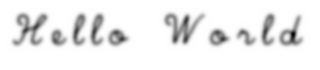
\includegraphics[width=\marginparwidth]{hello-world.png}}
``hello world''. Closing the window, or ctrl-c on the command line, will quit the application.

\section*{Integration with your favourite IDE}
We could now go ahead and start playing with the code in a text editor, however this really 
isn't recommended! Using a good Integrated Development Environment (IDE) with auto-completion will 
make your experience much better.

Maven integrates with all the popular IDEs. The OpenIMAJ developers all use Eclipse 
(\url{http://www.eclipse.org}) so that is what we're most familiar with, however we should be able 
to help getting it set up in a different IDE if you wish. 

Integration with Eclipse is quite simple. From the command line, inside the project directory, 
issue the command:
\begin{lstlisting}[language=bash]
mvn eclipse:eclipse
\end{lstlisting}
This will generate Eclipse project files in the same directory. In Eclipse you can then import 
the project into the Eclipse workspace (File>import..., choose ``Existing projects into workspace'', 
select the project directory, make sure ``Copy projects into workspace'' is \textbf{unchecked}, then click
 ``Finish''). The project should then appear in the workspace and you'll be able to look at the 
App.java file that was generated by the archetype.

\textbf{IMPORTANT} By default Eclipse doesn't know about Maven and its repositories of jars. When you 
first import an OpenIMAJ project into Eclipse it will have errors. You can fix this by adding 
a new Java classpath variable (\verb+Eclipse>Preferences>Java>+ \verb+Build Path>Classpath Variables+) 
called \verb+M2_REPO+. The value of this variable is the location of your \verb+.m2/repository+ directory. 
\marginpar{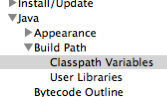
\includegraphics[width=\marginparwidth]{classpath.png}}
For Unix systems this is usually found in your home directory, for Windows systems it is found 
in \verb+C:\Documents and+ \verb+Settings\<user>\+.

Once you've opened the \verb+App.java+ file in Eclipse, you can right-click on it and select 
\verb+Run as>Java Application+ to run it from within Eclipse. 
\marginpar{
\includegraphics[width=\marginparwidth]{runas2.png}}

\section*{Exercises}
\subsection{Exercise 1: Playing with the sample application}
Take a look at the App.java from within your IDE. Can you modify the code to render something 
other than ``hello world'' in a different font and colour?

\chapter{Processing your first image}
In this section we'll start with the ``hello world'' app and show you how you can load an image, 
perform some basic processing on the image, draw some stuff on your image and then display your 
results.

Loading images into Java is usually a horrible experience. Using Java \verb+ImageIO+, one can use the 
\verb+read()+ method to create a \verb+BufferedImage+ object. Unfortunately the \verb+BufferedImage+ 
object hides the fact that it is (and in fact all digital raster images are) simply arrays of pixel 
values. A defining philosophy of OpenIMAJ is to \emph{keep things simple} which in turn means in OpenIMAJ 
images are as close as one can get to being \textbf{just arrays of pixel values}.

To read and write images in OpenIMAJ we use the \verb+ImageUtilities+ class. In the \verb+App.java+ 
class file remove the sample code within the main method and add the following line:
\begin{lstlisting}[language=java]
MBFImage image = ImageUtilities.readMBF(
       new File("file.jpg"));
\end{lstlisting}
For this tutorial, read the image from the following URL:
\begin{lstlisting}[language=java]
MBFImage image = ImageUtilities.readMBF(
    new URL("http://dl.dropbox.com/u/8705593/sinaface.jpg"));
\end{lstlisting}
The \verb+ImageUtilities+ class provides the ability to read \verb+MBFImage+s and \verb+FImage+s. 
An \verb+FImage+ is a greyscale image which represents each pixel as a value between \verb+0+ and 
\verb+1+. An \verb+MBFImage+ is a multi-band version of the \verb+FImage+; under the hood it actually
contains a number \verb+FImage+ objects held in a list each representing a band of the image. 
What these bands represent is given by the image's public \verb+colourSpace+ field, which we 
can print as follows:
\begin{lstlisting}[language=java]
System.out.println(image.colourSpace);
\end{lstlisting}
If we run the code, we'll see that the image is an RGB image with three \verb+FImage+s representing 
the red, blue and green components of the image in that order.

You can display any OpenIMAJ image object using the \verb+DisplayUtilities+ class. In this example we display
the image we have loaded then we display the red channel of the image alone: 
\marginpar{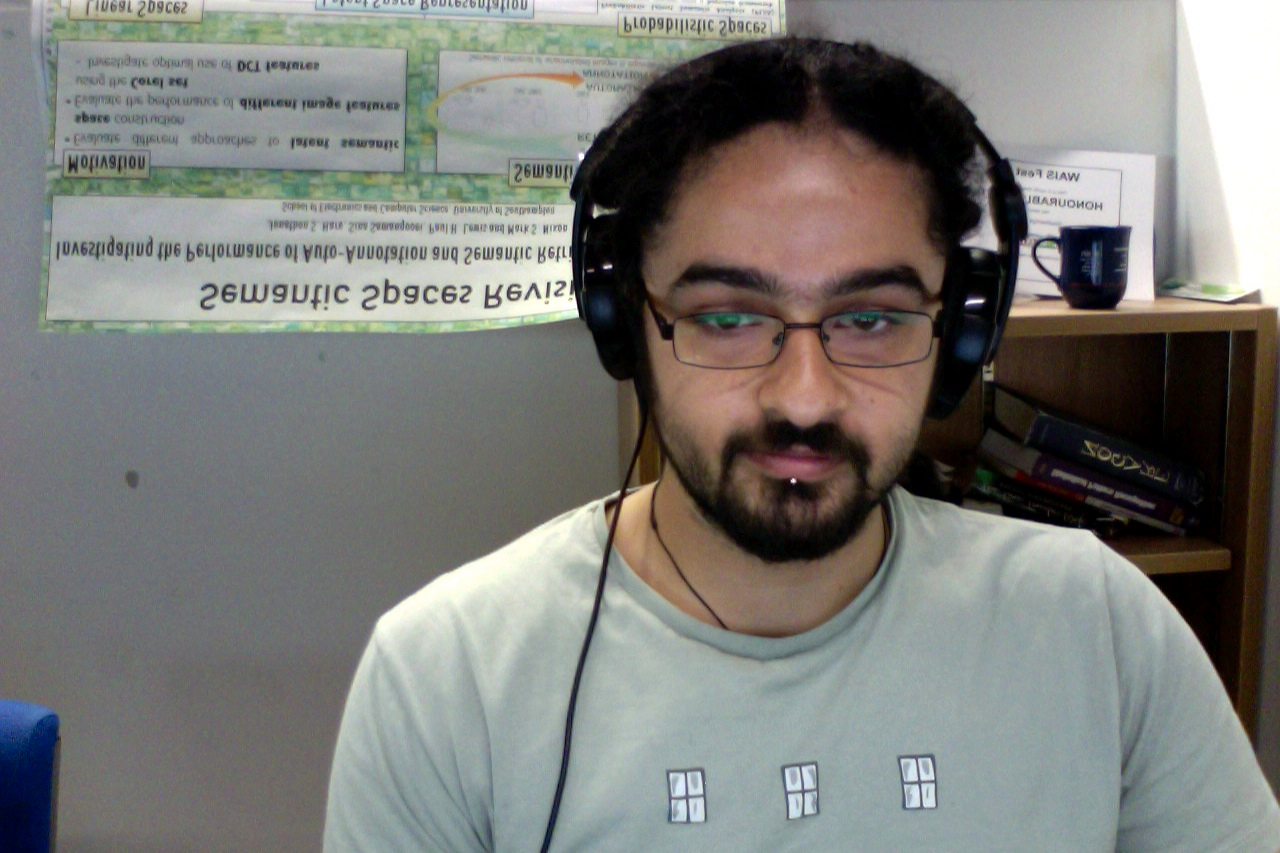
\includegraphics[width=\marginparwidth]{sinaface.png}}
\marginpar{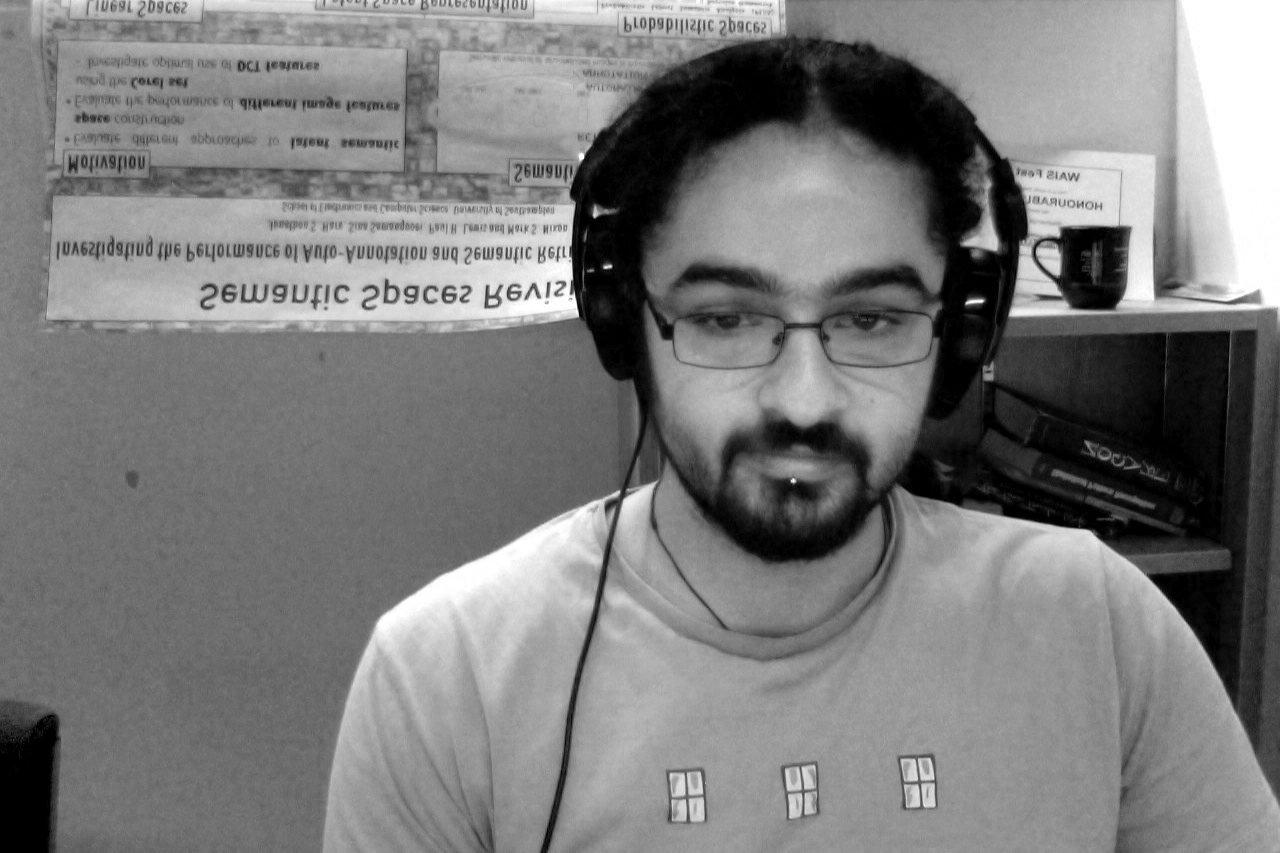
\includegraphics[width=\marginparwidth]{sinaface-rc.png}}
\begin{lstlisting}[language=java]
DisplayUtilities.display(image);
DisplayUtilities.display(
   image.getBand(0), "RedChannel");
\end{lstlisting}

In an image-processing library, images are no good unless you can do something to them. The most basic 
thing you can do to an image is fiddle with its pixels. In OpenIMAJ, as an image is just an array of 
floats, we make this is quite easy. Let's go through our colour image and set all its blue and green 
pixels to black: 
\begin{lstlisting}[language=java]
MBFImage clone = image.clone();
for (int y=0; y<image.getHeight(); y++) {
    for(int x=0; x<image.getWidth(); x++) {
        clone.getBand(1).pixels[y][x] = 0;
        clone.getBand(2).pixels[y][x] = 0;
    }
}
DisplayUtilities.display(clone);
\end{lstlisting}
Note that the first thing we do here is to \verb+clone+ the image to preserve the original image
for the remainder of the tutorial. The pixels in an \verb+FImage+ are held in a 2D float array. The rows 
of the image are held in the first array that, in turn, holds each of the column values for that 
row:  \verb+[y][x]+. By displaying this image we should see an image where two channels are black 
and one channel is not. This results in an image that looks rather red. 
\marginpar{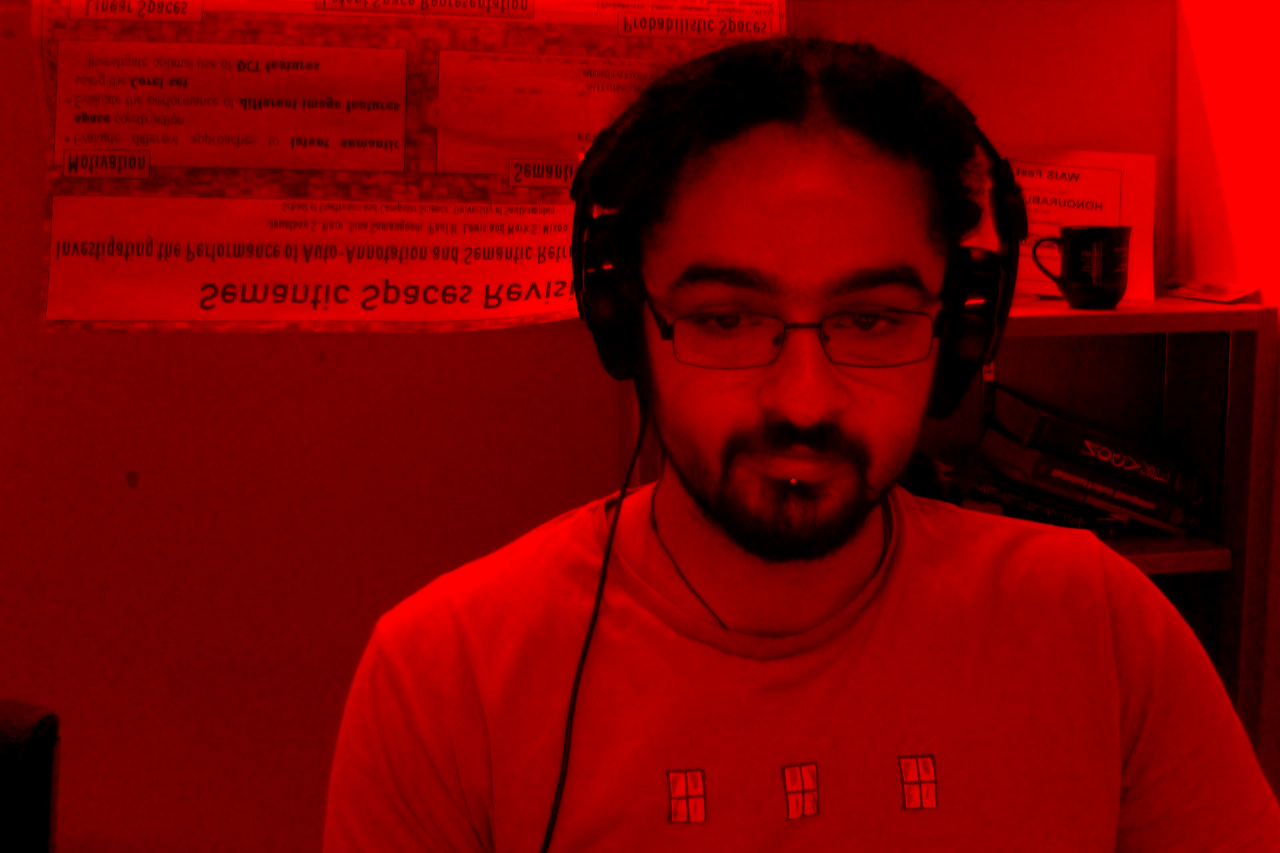
\includegraphics[width=\marginparwidth]{sinaface-red.png}}

Though it is helpful to sometimes get access to individual image pixels, OpenIMAJ provides a lot 
of methods to make things easier. For example, we could have done the above like this instead:
\begin{lstlisting}[language=java]
clone.getBand(1).fill(0f);
clone.getBand(2).fill(0f);
\end{lstlisting}

More complex image operations are wrapped up by OpenIMAJ processor interfaces: \verb+ImageProcessor+s, \verb+KernelProcessor+s,
\verb+PixelProcessor+s and \verb+GridProcessor+s. The distinction between these is how their algorithm works internally. The overarching similarity is that an image goes 
in and a processed image (or data) comes out. For example, a basic operation in image processing 
is \textbf{edge detection}. A popular edge detection algorithm is the \emph{Canny edge detector}. 
We can call the Canny edge detector like so:
\begin{lstlisting}[language=java]
image.processInplace(new CannyEdgeDetector2());
\end{lstlisting}
When applied to a colour image, each pixel of each band is replaced with the edge response at 
that point (for simplicity you can think of this as the difference between that pixel and its 
neighbouring pixels). If a particular edge is only strong in one band or another then that 
colour will be strong, resulting in the psychedelic colours you should see if you display 
the image:
\begin{lstlisting}[language=java]
DisplayUtilities.display(image);
\end{lstlisting}
\marginpar{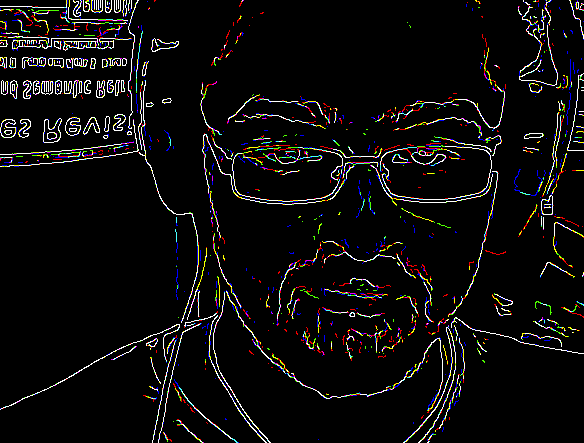
\includegraphics[width=\marginparwidth]{sinaface-canny.png}}

Finally, we can also draw on our image in OpenIMAJ. On every \verb+Image+ object there is a 
set of drawing functions that can be called to draw points, lines, shapes and text on 
images. Let's draw some speech bubbles on our image:
\begin{lstlisting}[language=java]
image.drawShapeFilled(new Ellipse(700f, 450f, 20f, 10f, 0f), RGBColour.WHITE);
image.drawShapeFilled(new Ellipse(650f, 425f, 25f, 12f, 0f), RGBColour.WHITE);
image.drawShapeFilled(new Ellipse(600f, 380f, 30f, 15f, 0f), RGBColour.WHITE);
image.drawShapeFilled(new Ellipse(500f, 300f, 100f, 70f, 0f), RGBColour.WHITE);
image.drawText("OpenIMAJ is", 425, 300, HersheyFont.ASTROLOGY, 20, RGBColour.BLACK);
image.drawText("Awesome", 425, 330, HersheyFont.ASTROLOGY, 20, RGBColour.BLACK);
DisplayUtilities.display(image);
\end{lstlisting}
Here we construct a series of ellipses (defined by their centre [x, y], axes 
[major, minor] and rotation) and draw them as white filled shapes. Finally, we draw 
some text on the image and display it.
\marginpar{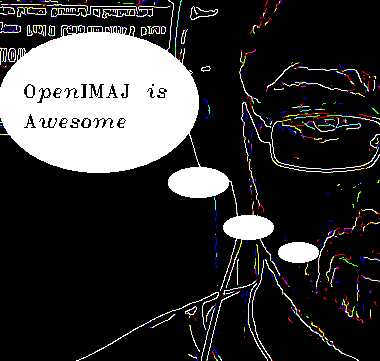
\includegraphics[width=\marginparwidth]{sinaface-awesome.png}}

\section*{Exercises}
\subsection*{Exercise 1: DisplayUtilities}
Opening lots of windows can waste time and space (for example if you wanted to view images on every 
iteration of a process within a loop). In OpenIMAJ we provide a facility to open a 
\emph{named display} so that was can reuse the display referring to it by name. Try to do this with all the 
images we display in this tutorial. Only 1 window should open for the whole tutorial.
\subsection*{Exercise 2: Drawing}
Those speech bubbles look rather plain; why not give them a nice border?

\chapter{Introduction to clustering, segmentation and connected components}
In this tutorial we'll create an application that demonstrates how an image can be 
broken into a number of regions. The process of separating an image into regions, 
or segments, is called \textbf{segmentation}. Segmentation is a widely studied area in 
computer vision. Researchers often try to optimise their segmentation algorithms 
to try and separate the \textbf{objects} in the image from the \textbf{background}.

To get started, create a new OpenIMAJ project using the Maven archetype, 
import it into your IDE, and delete the sample code from within the generated 
\verb+main()+ method of the \verb+App+ class. In the \verb+main()+ method, 
start by adding code to load an image (choose your own image):
\begin{lstlisting}[language=java]
MBFImage input = ImageUtilities.readMBF(
   new URL("http://..."));
\end{lstlisting}

To segment our image we are going to use a machine 
\marginpar{K-Means initialises cluster centroids with randomly selected data points
and then iteratively assigns the data points to their closest cluster and updates 
the centroids to the mean of the respective clusters data points} 
learning technique called 
\textbf{clustering}. Clustering algorithms automatically group similar things together. In our 
case, we'll use a popular clustering algorithm called \textbf{K-Means} clustering to group 
together all the similar colours in our image. Each group of similar colours is 
known as a \textbf{class}. The K-means clustering algorithm requires you set the number 
of classes you wish to find \textbf{a priori} (i.e. beforehand). 

Colours in our input image are represented in \textbf{RGB colour space}; that is each pixel is 
represented as three numbers corresponding to a red, green and blue value. In order 
to measure the similarity of a pair of colours the ``distance'' between the colours in 
the colour space can be measured. \marginpar{The Euclidean distance is the straight-line 
distance between two points.} Typically, the distance measured is the \textbf{Euclidean} 
distance. Unfortunately, distances in RGB colour space do not reflect what humans perceive as 
similar/dissimilar colours. In order to work-around this problem it is common to transform 
an image into an alternative colour space. The \textbf{Lab colour space} (pronounced as 
separate letters, L A B) is specifically designed so that the Euclidean distance between 
colours closely matches the perceived similarity of a colour pair by a human observer.

\pagebreak
To start our implementation, we'll first apply a colour-space transform to the image:
\begin{lstlisting}[language=java]
input = ColourSpace.convert(input,ColourSpace.CIE_Lab);
\end{lstlisting}
We can then construct the K-Means algorithm:
\begin{lstlisting}[language=java]
FastFloatKMeans cluster = new FastFloatKMeans(3,2,true);
\end{lstlisting}
The first parameter is the dimensionality of the space (3 in this case corresponding 
to the \textbf{L}, \textbf{a}, and \textbf{b} dimensions of the colour vectors). The second 
argument is the number of clusters or classes we wish the algorithm to generate. The final 
boolean flag indicates whether the underlying algorithm should be the ``exact'' K-means algorithm (true) or an 
\textbf{approximate} algorithm (false). The approximate algorithm is much faster than the exact 
algorithm when there is very high-dimensional data; in this case, with only three dimensions, 
the approximate algorithm is not required. The OpenIMAJ K-Means implementation is 
multithreaded and automatically takes advantage of all the processing power it can obtain.

The FastFloatKMeans algorithm takes its input as an array of floating point vectors
(\verb+float[][]+). We can flatten the pixels of an image into the required form using the 
\verb+getPixelVectorNative()+ method:
\begin{lstlisting}[language=java]
float[][] imageData = input.getPixelVectorNative(new float[input.getWidth() * input.getHeight()][3]);
\end{lstlisting}
The K-Means algorithm can then be run to group all the pixels into the requested number of classes:
\begin{lstlisting}[language=java]
cluster.cluster(imageData);
\end{lstlisting}
Each class or cluster produced by the K-Means algorithm has an index, starting from 0. Each class is 
represented by its centroid (the average location of all the points belonging to the class). We can 
print the coordinates of each centroid:
\begin{lstlisting}[language=java]
float[][] centroids = cluster.getCentroids();
for (float[] fs : centroids) {
    System.out.println(Arrays.toString(fs));
}
\end{lstlisting}
Now is a good time to test the code. Running it should print the (\verb+L, a, b+) coordinates of each 
of the classes.

We can now use a \verb+HardAssigner+ to assign each pixel in our image to its respective 
class using the centroids learned during the \verb+FastFloatKMeans+. This is a process known as \textbf{classification}. There are a number of different \verb+HardAssigner+s, however, \verb+FastFloatKMeans+ has a method called \verb+defaultHardAssigner()+ which will return an assigner fit for our purposes. \verb+HardAssigner+s have a method called \verb+assign()+ which takes a vector (the \verb+L, a, b+ value of a single pixel) and 
returns the index of the class that it belongs to. We'll start by creating an image that 
visualises the pixels and their respective classes by replacing each pixel in the input image 
with the centroid of its respective class:
\begin{lstlisting}[language=java]
HardAssigner<float[],?,?> assigner = cluster.defaultHardAssigner();
for (int y=0; y<input.getHeight(); y++) {
    for (int x=0; x<input.getWidth(); x++) {
        float[] pixel = input.getPixelNative(x, y);
        int centroid = assigner.assign(pixel);
        input.setPixelNative(x, y, centroids[centroid]);
    }
}
\end{lstlisting}
We can then display the resultant image. Note that we need to convert the image back to RGB 
colour space for it to display properly:
\begin{lstlisting}[language=java]
input = ColourSpace.convert(input, ColourSpace.RGB);
DisplayUtilities.display(input);
\end{lstlisting}
Running the code will display an image that looks a little like the original image but with 
as many colours as there are classes. 
\marginpar{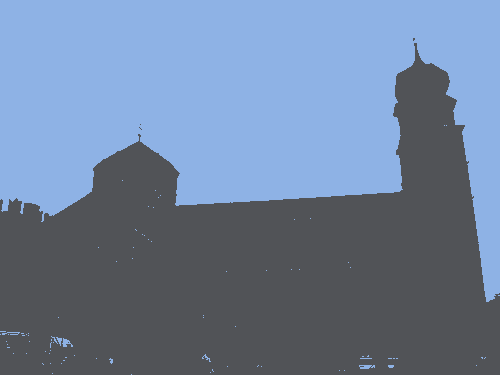
\includegraphics[width=\marginparwidth]{kmeans.png}}

To actually produce a segmentation of the image we need to group together all pixels with 
the same class that are touching each other. Each set of pixels representing a segment is 
often referred to as a \textbf{connected component}. Connected components in OpenIMAJ are
modelled by the \verb+ConnectedComponent+ class.

The \verb+GreyscaleConnectedComponentLabeler+ class can be used to find the connected components:
\begin{lstlisting}[language=java]
GreyscaleConnectedComponentLabeler labeler = new GreyscaleConnectedComponentLabeler();
List<ConnectedComponent> components = labeler.findComponents(input.flatten());
\end{lstlisting}
Note that the \verb+GreyscaleConnectedComponentLabeler+ 
\marginpar{OpenIMAJ also contains a class called \texttt{ConnectedComponent}-\texttt{Labeler} which can
only be used on \textbf{binary} (i.e. pure black and white) \texttt{FImage}s.} 
only processes greyscale images 
(the \verb+FImage+ class) and not the colour image (\verb+MBFImage+ class) that we created. 
The \verb+flatten()+ method on \verb+MBFImage+ merges the colours into grey values by 
averaging their RGB values.

The \verb+ConnectedComponent+ class has many useful methods for extracting information 
about the shape of the region. Lets draw an image with the components numbered on it. We'll use the 
centre of mass of each region to position the number and only render numbers for regions that 
are over a certain size (50 pixels in this case):
\begin{lstlisting}[language=java]
int i = 0;
for (ConnectedComponent comp : components) {
    if (comp.calculateArea() < 50) 
        continue;
    input.drawText("Point:" + (i++), comp.calculateCentroidPixel(), HersheyFont.TIMES_MEDIUM,20);
}
\end{lstlisting}
Finally, we can display the image with the labels:
\begin{lstlisting}[language=java]
DisplayUtilities.display(input);
\end{lstlisting}
\marginpar{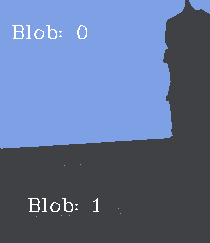
\includegraphics[width=\marginparwidth]{segmented.png}}

\pagebreak
\section*{Exercises}
\subsection*{Exercise 1: The PixelProcessor}
Rather than looping over the image pixels using two for loops, it is possible to use a 
\verb+PixelProcessor+ to accomplish the same task:
\begin{lstlisting}[language=java]
image.processInline(new PixelProcessor<Float[]>() {
    Float[] processPixel(Float[] pixel, Number[]...otherpixels) {
        ...
    }
});
\end{lstlisting}
Can you re-implement the loop that replaces each pixel with its class centroid 
using a \verb+PixelProcessor+? 

What are the advantages and disadvantages of using a \verb+PixelProcessor+?

\subsection*{Exercise 2: A real segmentation algorithm}
The segmentation algorithm we just implemented can work reasonably well, but is rather na\"ive. OpenIMAJ contains an 
implementation of a popular segmentation algorithm called the \verb+FelzenszwalbHuttenlocherSegmenter+. 

Try using the \verb+FelzenszwalbHuttenlocherSegmenter+ for yourself and see how it compares to the 
basic segmentation algorithm we implemented. You can use the \verb+SegmentationUtilities.renderSegments()+ 
static method to draw the connected components produced by the segmenter.


\chapter{Processing video}
In this section we'll show you how to deal with videos using OpenIMAJ. We provide a 
set of tools for loading, displaying and processing various kinds of video. 

All videos in OpenIMAJ are subtypes of the \verb+Video+ class. This class is typed 
on the type of underlying frame. In this case, let's create a video which holds coloured frames:
\begin{lstlisting}[language=java]
Video<MBFImage> video;
\end{lstlisting}

Exactly what kind of video is loaded depends on what you want to do. To load a video from a file
we use the \textbf{Xuggle} library which internally uses \verb+ffmpeg+. Let's load a video 
from a file (which you can download from here: \url{http://dl.dropbox.com/u/8705593/keyboardcat.flv}).

First you'll need to install Xuggle. Go to http://www.xuggle.com/xuggler/downloads/ and pick your platform 
then follow the instructions.

While this is downloading, let's write the code.
\marginpar{The \texttt{XuggleVideo} class also has a constructor that lets you pass a URL to a video on the web without downloading it first.}
If we want to load a video from a file we use a \verb+XuggleVideo+ object: 
\begin{lstlisting}[language=java]
video = new XuggleVideo(new File("/path/to/keyboardcat.flv"));
\end{lstlisting}

If your computer has a webcam, OpenIMAJ also supports live video input. These are called capture 
devices and you can use one through the \verb+VideoCapture+ class:
\begin{lstlisting}[language=java]
video = new VideoCapture(320,240);
\end{lstlisting}
This will find the first video capture device attached to your system and render it as closely to 
$320\times240$ pixels as it can. To select a specific device you can use the alternative constructors
and use the \verb+VideoCapture.getVideoDevices()+ static method to obtain the available devices.

Note that webcam capture does not require a Xuggle install and is completely built into OpenIMAJ.

To see if either of these kinds of video work, we can use \verb+VideoDisplay+ to display videos. This is 
achieved using the static function calls in \verb+VideoDisplay+ (which mirror those found in 
\verb+DisplayUtilities+ for images) like so:
\begin{lstlisting}[language=java]
VideoDisplay<MBFImage> display = VideoDisplay.createVideoDisplay(video);
\end{lstlisting}

Simply by creating a display, the video starts and plays. You can test this by running 
your app after Xuggle is installed. 
\marginpar{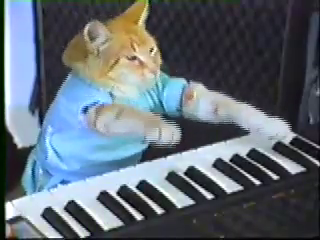
\includegraphics[width=\marginparwidth]{frame.png}}

\textbf{Note:} If you're using Linux or MacOSX, you might encounter an error trying to run this from Eclipse. 
This is due to library dependencies on Xuggle. To fix this, in Eclipse go to the run configuration 
(\verb+Run>Run Configurations+). Once here click the \verb+Environments+ tab. Add a new environment 
variable called \verb+DYLD_LIBRARY_PATH+ on MacOSX or \verb+LD_LIBRARY_PATH+ on Linux and set this to 
the location of the \verb+xuggler/lib+ directory (this is likely to be \verb+/usr/local/xuggler/lib+
if you went with the default Xuggle install options).

As with images, displaying them is nice but what we really want to do is process the frames of 
the video in some way. This can be achieved in various ways; firstly videos are \verb+Iterable+, so you can 
do something like this to iterate through every frame and process it:
\begin{lstlisting}[language=java]
for (MBFImage mbfImage : video) {
    DisplayUtilities.displayName(mbfImage.process(new CannyEdgeDetector2()), "videoFrames");
}
\end{lstlisting}
Here we're applying a Canny edge detector to each frame and displaying the frame in a named window. Another 
approach, which ties processing to image display automatically, is to use an event driven technique:
\marginpar{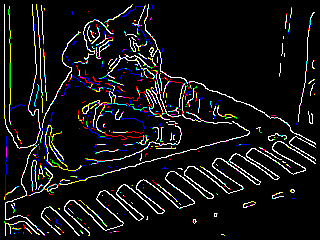
\includegraphics[width=\marginparwidth]{frame-canny.png}}
\begin{lstlisting}[language=java]
VideoDisplay<MBFImage> display = VideoDisplay.createVideoDisplay(video);
display.addVideoListener(
  new VideoDisplayListener<MBFImage>() {
    @Override
    public void beforeUpdate(MBFImage frame) {
        frame.processInline(new CannyEdgeDetector2());
    }

    @Override
    public void afterUpdate(VideoDisplay<MBFImage> display) {
    }
  });
\end{lstlisting}

These \verb+VideoDisplayListener+s are given video frames before they are rendered and they are handed the 
video display after the render has occurred. The benefit of this approach is that functionality such as 
looping, pausing and stopping the video is given to you for free by the \verb+VideoDisplay+ class. 

\section*{Exercises}
\subsection*{Exercise 1: Applying different types of image processing to the video}
Try a different processing operation and see how it affects the frames of your video.

\chapter{Finding faces}
OpenIMAJ contains a set of classes that contain implementations of some of the state-of-the-art face 
detection and recognition algorithms. These classes are provided as a sub-project of the OpenIMAJ 
code-base called \verb+faces+. The OpenIMAJ maven archetype adds the face library as a dependency and 
so we can start building face detection applications straight away.

Create a new application using the quick-start archetype (see tutorial 1) and import it into your IDE. 
If you look at the \verb+pom.xml+ file you will see that the \verb+faces+ dependency from OpenIMAJ is 
already included. As you've already done the video-processing tutorial, we'll try to find faces within 
the video that your webcam produces. If you don't have a webcam, follow the video tutorial on how to 
use video from a file instead.

Start by removing the code from the main method of the \verb+App.java+ class file. Then create a video 
capture object and a display to show the video. Create a listener on the video display to which we can 
hook our face finder. The code is below, but check out the previous tutorial on video processing if 
you're not sure what it means.
\begin{lstlisting}[language=java]
VideoCapture vc = new VideoCapture( 320, 240 );
VideoDisplay<MBFImage> vd = VideoDisplay.createVideoDisplay( vc );
vd.addVideoListener( 
  new VideoDisplayListener<MBFImage>() {
    @Override
    public void beforeUpdate( MBFImage frame ) {
    }

    @Override
    public void afterUpdate( VideoDisplay<MBFImage> display ) {
    }
  });
\end{lstlisting}
For finding faces in images (or in this case video frames) we use a face detector. The \verb+FaceDetector+ 
interface provides the API for face detectors and there are currently two implementations within OpenIMAJ - 
the \verb+HaarCascadeDetector+ and the \verb+SandeepFaceDetector+. The \verb+HaarCascadeDetector+
is considerably more robust than the \verb+SandeepFaceDetector+, so we'll use that.

In the \verb+beforeUpdate()+ method, instantiate a new \verb+HaarCascadeDetector+. The constructor takes 
the minimum size in pixels that a face can be detected at. For now, set this to \verb+40+ pixels:
\begin{lstlisting}[language=java]
FaceDetector<DetectedFace,FImage> fd = new HaarCascadeDetector(40);
\end{lstlisting}

Like all \verb+FaceDetector+ implementations, the \verb+HaarCascadeDetector+ has a method \verb+detectFaces()+
which takes an image. Because the \verb+HaarCascadeDetector+ uses single band images, we must convert 
our multi-band colour image into a single band image. To do this we can use the \verb+Transforms+ utility 
class that contains some static methods for converting images. The \verb+calculateIntensity()+ method 
will do just fine. Note that functionally the \verb+calculateIntensity()+ method does the same thing 
as the \verb+flatten()+ method we used earlier when used on RGB images.
\begin{lstlisting}[language=java]
List<DetectedFace> faces = fd.detectFaces(Transforms.calculateIntensity(frame));
\end{lstlisting}
The \verb+detectFaces()+ method returns a list of \verb+DetectedFace+ objects which contain 
information about the faces in the image. From these objects we can get the rectangular 
bounding boxes of each face and draw them back into our video frame. As we're doing all 
this in our \verb+beforeUpdate()+ method, the video display will end up showing the 
bounding boxes on the displayed video. If you run the code and you have a webcam attached,
you should see yourself with a box drawn around your face. The complete code is shown below:
\begin{lstlisting}[language=java]
FaceDetector<DetectedFace,FImage> fd = new HaarCascadeDetector(40);
List<DetectedFace> faces =
            fd.detectFaces( Transforms.calculateIntensity(frame));

for( DetectedFace face : faces ) {
    frame.drawShape(face.getBounds(), RGBColour.RED);
}
\end{lstlisting}
\marginpar{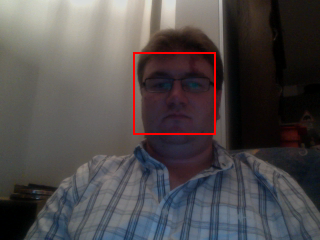
\includegraphics[width=\marginparwidth]{face-bounds.png}}
OpenIMAJ has other face detectors which go a bit further than just finding the face. 
The \verb+FKEFaceDetector+ finds facial keypoints (the corners of the eyes, nose and mouth) 
and we can use this detector instead simply by instantiating that object instead of the 
\verb+HaarCascadeDetector+. The \verb+FKEFaceDetector+ returns a slightly different object 
for each detected face, called a \verb+KEDetectedFace+. The \verb+KEDetectedFace+ object 
contains the extra information about where the keypoints in the face are located. 
The lines of our code to instantiate the detector and detect faces can now be changed to 
the following:
\begin{lstlisting}[language=java]
FaceDetector<KEDetectedFace,FImage> fd = new FKEFaceDetector();
List<KEDetectedFace> faces = fd.detectFaces( Transforms.calculateIntensity( frame ) );
\end{lstlisting}
If you run the demo now, you will see exactly the sameas before, as the \verb+FKEFaceDetector+ 
still detects bounding boxes. It may be running a bit slower though, as there is much more 
processing going on - we're just not seeing the output of it! So, let's plot the facial keypoints.

To get the keypoints use \verb+getKeypoints()+ on the detected face. Each keypoint has a 
position (public field) which is relative to the face, so we'll need to translate the 
point to the position of the face within the video frame before we plot the points. 
To do that we can use the \verb+translate()+ method of the \verb+Point2d+ class
and the \verb+minX()+ and \verb+minY()+ methods of the \verb+Rectangle+ class.

\section*{Exercises}
\subsection*{Exercise 1: Drawing facial keypoints}
Use the information above to plot the facial keypoints on the video.
\marginpar{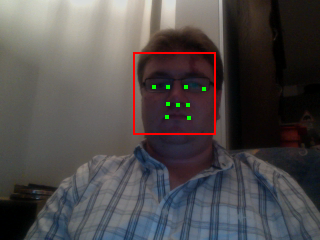
\includegraphics[width=\marginparwidth]{face-points.png}}

\subsection*{Exercise 2: Speech bubbles}
Try and take the speech bubble from the previous image tutorial and make it come from the mouth 
in the video. \textbf{Hints:} use \verb+getKeypoint(FacialKeypointType)+ to get the keypoint 
of the left corner of the mouth and plot the ellipses depending on that point. You may need to 
use smaller ellipses and text if your video is running at 320x240.
\marginpar{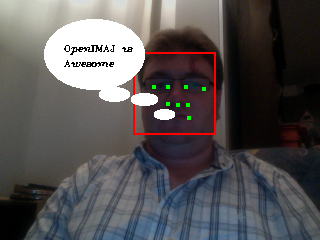
\includegraphics[width=\marginparwidth]{face-awesome.png}}

\chapter{Global image features}
The task in this tutorial is to understand how we can extract numerical representations from images 
and how these numerical representations can be used to provide similarity measures between images, 
so that we can, for example, find the most similar images from a set.

As you know, images are made up of pixels which are basically numbers that represent a colour. 
This is the most basic form of numerical representation of an image. However, we can do calculations 
on the pixel values to get other numerical representations that mean different things. In general, 
these numerical representations are known as \textbf{feature vectors} and they represent particular 
\textbf{features}.

Let's take a very common and easily understood type of feature. It's called a colour histogram and 
it basically tells you the proportion of different colours within an image (e.g. 90\% red, 5\% green, 
3\% orange, and 2\% blue). As pixels are represented by different amounts of red, green and blue we 
can take these values and accumulate them in our histogram (e.g. when we see a red pixel we add 1 
to our `red pixel count' in the histogram). 

A histogram can accrue counts for any number of colours in any number of dimensions but the usual 
is to split the red, green and blue values of a pixel into a smallish number of `bins' into which the 
colours are thrown.  This gives us a three-dimensional cube, where each small cubic bin is accruing 
counts for that colour.

OpenIMAJ contains a multidimensional \verb+Histogram+ implementation that is constructed using the number 
of bins required in each dimension. For example:
\begin{lstlisting}[language=java]
Histogram histogram = new Histogram( 4, 4, 4 );
\end{lstlisting}
This code creates a histogram that has 64 ($4\times4\times4$) bins. However, this data structure does not do 
anything on its own. The \verb+HistogramModel+ class provides a means for creating a \verb+Histogram+ 
from an image.  The \verb+HistogramModel+ class assumes the image has been normalised and returns a normalised histogram:
\begin{lstlisting}[language=java]
HistogramModel model = new HistogramModel( 4, 4, 4 );
model.estimateModel( image );
Histogram histogram = model.histogram;
\end{lstlisting}

You can print out the histogram to see what sort of numbers you get for different images. 
Let's load in 3 images then generate and store the histograms for them:
\marginpar{
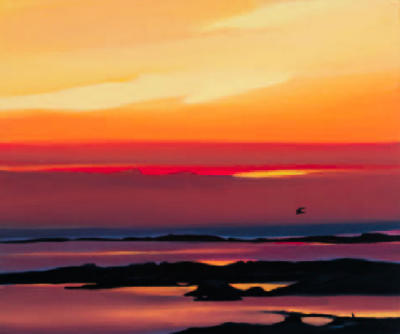
\includegraphics[width=\marginparwidth]{hist1.jpg}
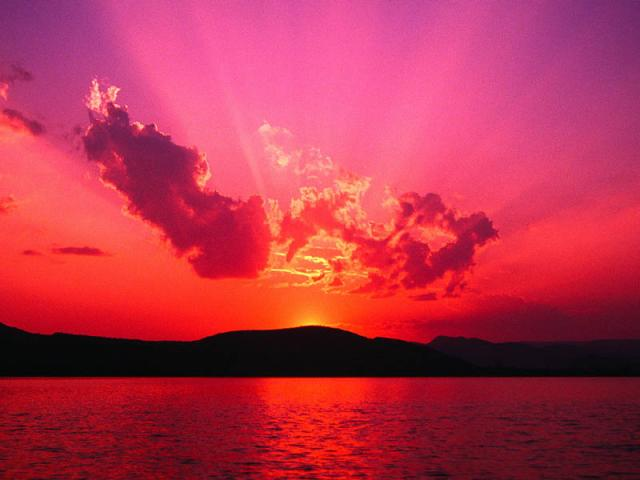
\includegraphics[width=\marginparwidth]{hist2.jpg}
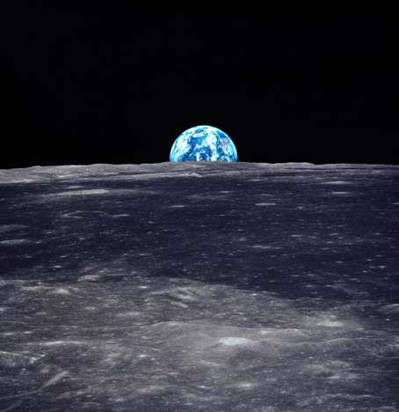
\includegraphics[width=\marginparwidth]{hist3.jpg}
}
\begin{lstlisting}[language=java]
URL[] imageURLs = new URL[] {
   new URL( "http://users.ecs.soton.ac.uk/dpd/projects/openimaj/tutorial/hist1.jpg" ),
   new URL( "http://users.ecs.soton.ac.uk/dpd/projects/openimaj/tutorial/hist2.jpg" ), 
   new  URL( "http://users.ecs.soton.ac.uk/dpd/projects/openimaj/tutorial/hist3.jpg" ) 
};
List<Histogram> histograms = new ArrayList<Histogram>();
for( URL u : imageURLs ) {
    HistogramModel model = new HistogramModel(4, 4, 4);
    model.estimateModel(ImageUtilities.readMBF(u));
    histograms.add( model.histogram );
}
\end{lstlisting}
We now have a list of histograms from our images.  The \verb+Histogram+ class extends a 
class called the \verb+MultidimensionalDoubleFV+ which is a feature vector represented 
by multidimensional set of double precision numbers.  This class provides us with a 
\verb+compare()+ method which allows comparison between two multidimensional sets of 
doubles. This method takes the other feature vector to compare against and a comparison 
method which is implemented in the \verb+DoubleFVComparison+ class.

So, we can compare two histograms using the Euclidean distance measure like so:
\begin{lstlisting}[language=java]
double distanceScore = histogram1.compare( histogram2, DoubleFVComparison.EUCLIDEAN );
\end{lstlisting}
This will give us a score of how similar (or dissimilar) the histograms are. It's useful
to think of the output score as a \textbf{distance} apart in space. Two very similar histograms 
will be very close together so have a small distance score, whereas two dissimilar 
histograms will be far apart and so have a large distance score.

The Euclidean distance measure is symmetric (that is, if you compare \verb+histogram1+ to 
\verb+histogram2+ you will get the same score if you compare \verb+histogram2+ to 
\verb+histogram1+) so we can compare all the histograms with each other in a simple, 
efficient, nested loop:
\begin{lstlisting}[language=java]
for( int i = 0; i < histograms.size(); i++ ) {
    for( int j = i; j < histograms.size(); j++ ) {
        double distance = histograms.get(i).compare( histograms.get(j), DoubleFVComparison.EUCLIDEAN );
    }
}
\end{lstlisting}

\section*{Exercises}
\subsection*{Exercise 1: Finding and displaying similar images}
Which images are most similar?  Does that match with what you expect if you look at the 
images?  Can you make the application display the two most similar images that aren't the same?

\subsection*{Exercise 2: Exploring comparison measures}
\raggedright
What happens when you use a different comparison measure (such as 
\verb+DoubleFVComparison.INTERSECTION+)?

\chapter{SIFT and feature matching}
In this tutorial we'll look at how to compare images to each other. Specifically, we'll use a
popular \textbf{local feature descriptor} called \textbf{SIFT} to extract some \emph{interesting points} 
from images and describe them in a standard way. Once we have these local features and their 
descriptions, we can match local features to each other and therefore compare images to each 
other, or find a visual query image within a target image, as we will do in this tutorial.

Firstly, lets load up a couple of images. Here we have a magazine and a scene containing the 
magazine:
\begin{lstlisting}[language=java]
MBFImage query = ImageUtilities.readMBF(new 
                             URL("http://dl.dropbox.com/u/8705593/query.jpg"));
\end{lstlisting}
\marginpar{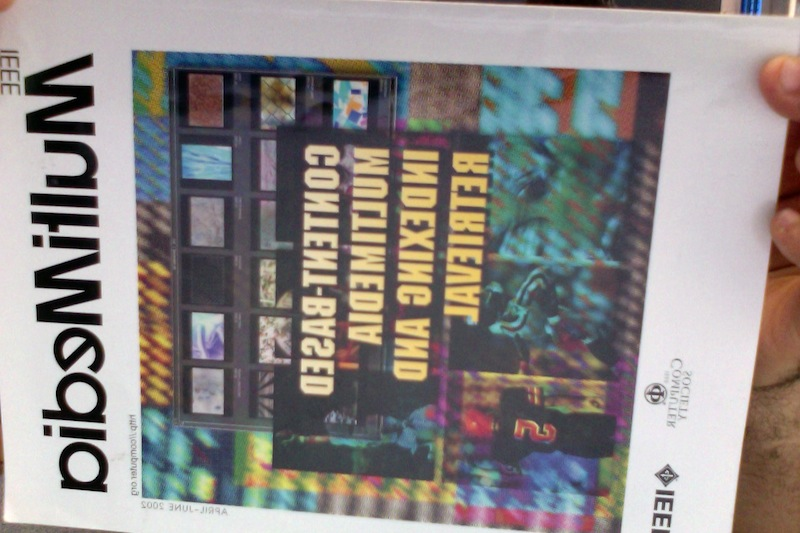
\includegraphics[width=\marginparwidth]{query.jpg}}
\begin{lstlisting}[language=java]
MBFImage target = ImageUtilities.readMBF(new 
                             URL("http://dl.dropbox.com/u/8705593/target.jpg"));
\end{lstlisting}
\marginpar{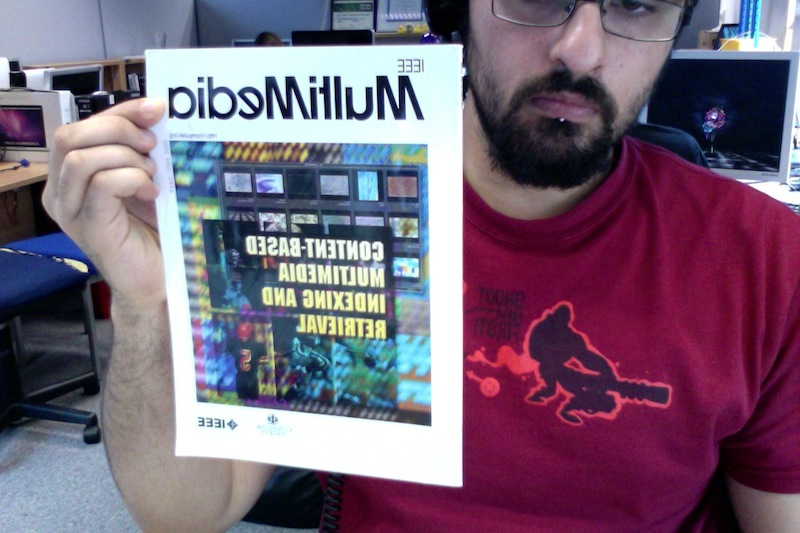
\includegraphics[width=\marginparwidth]{target.jpg}}

The first step is feature extraction. We'll use the \textbf{difference-of-Gaussian} feature detector 
which we describe with a \textbf{SIFT descriptor}. The features we find are described in a way which 
makes them invariant to size changes, rotation and position. These are quite powerful features and 
are used in a variety of tasks. The standard implementation of SIFT in OpenIMAJ can be found in the 
\verb+DoGSIFTEngine+ class:
\begin{lstlisting}[language=java]
DoGSIFTEngine engine = new DoGSIFTEngine();	
LocalFeatureList<Keypoint> queryKeypoints = engine.findFeatures(query.flatten());
LocalFeatureList<Keypoint> targetKeypoints = engine.findFeatures(target.flatten());
\end{lstlisting}
Once the engine is constructed, we can use it to extract \verb+Keypoint+ objects from our images. 
The \verb+Keypoint+ class contain a public field called \verb+ivec+ which, in the case
of a standard SIFT descriptor is a 128 dimensional description of a patch of pixels around a 
detected point. Various distance measures can be used to compare \verb+Keypoint+s to \verb+Keypoint+s.

The challenge in comparing \verb+Keypoint+s is trying to figure out which \verb+Keypoint+s match 
between \verb+Keypoint+s from some query image and those from some target. The most basic approach 
is to take a given \verb+Keypoint+ in the query and find the \verb+Keypoint+ that is closest in the 
target. A minor improvement on top of this is to disregard those points which match well with MANY
other points in the target. Such point are considered non-descriptive. Matching can be achieved in 
OpenIMAJ using the \verb+BasicMatcher+. Next we'll construct and setup such a matcher:
\begin{lstlisting}[language=java]
LocalFeatureMatcher<Keypoint> matcher = new BasicMatcher<Keypoint>(80);
matcher.setModelFeatures(queryKeypoints);
matcher.findMatches(targetKeypoints);
\end{lstlisting}
We can now draw the matches between these two images found with this basic matcher using the 
\verb+MatchingUtilities+ class:
\begin{lstlisting}[language=java]
MBFImage basicMatches = MatchingUtilities.drawMatches(query, target, matcher.getMatches(), RGBColour.RED);
DisplayUtilities.display(basicMatches);
\end{lstlisting}
\marginpar{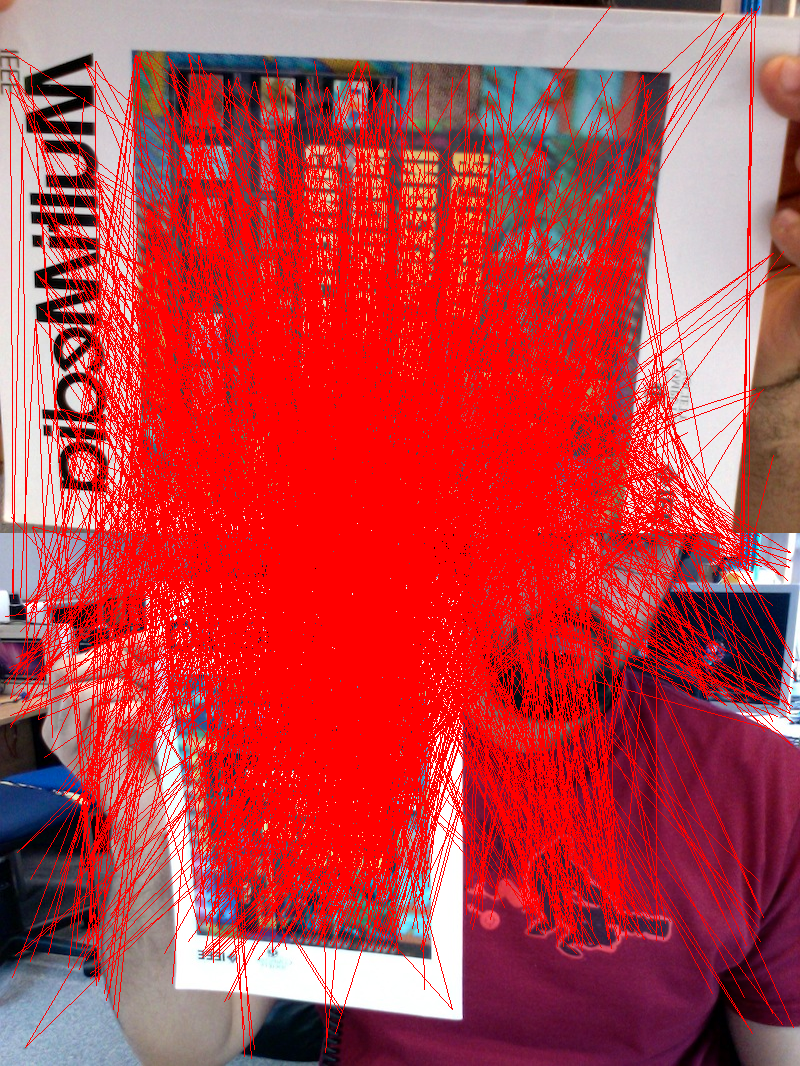
\includegraphics[width=\marginparwidth]{matches.png}}
As you can see, the basic matcher finds many matches, many of which are clearly incorrect. A more advanced 
approach is to filter the matches based on a given geometric model. One way of achieving this in OpenIMAJ 
is to use a \verb+ConsistentLocalFeatureMatcher+ which given an internal matcher, a geometric model and 
a model fitter, finds which matches given by the internal matcher are consistent with respect to the model
and are therefore likely to be correct.

To demonstrate this, we'll use an algorithm called Random Sample Consensus (RANSAC) to fit a geometric model
\marginpar{An Affine transform models the transformation between two parallelograms.}
called an \textbf{Affine transform} to the initial set of matches. This is achieved by iteratively 
selecting a random set of matches, learning a model from this random set and then testing the 
remaining matches against the learnt model. 

We'll now set up our model, our RANSAC model fitter and our consistent matcher:
\begin{lstlisting}[language=java]
AffineTransformModel fittingModel = new AffineTransformModel(5);
RANSAC<Point2d, Point2d> ransac = new RANSAC<Point2d, Point2d>(fittingModel, 1500, new RANSAC.PercentageInliersStoppingCondition(0.5), true);

matcher = new ConsistentLocalFeatureMatcher2d<Keypoint>(
  new FastBasicKeypointMatcher<Keypoint>(8), ransac);

matcher.setModelFeatures(queryKeypoints);
matcher.findMatches(targetKeypoints);
MBFImage consistentMatches = MatchingUtilities.drawMatches(query, target, matcher.getMatches(), RGBColour.RED);
\end{lstlisting}
\marginpar{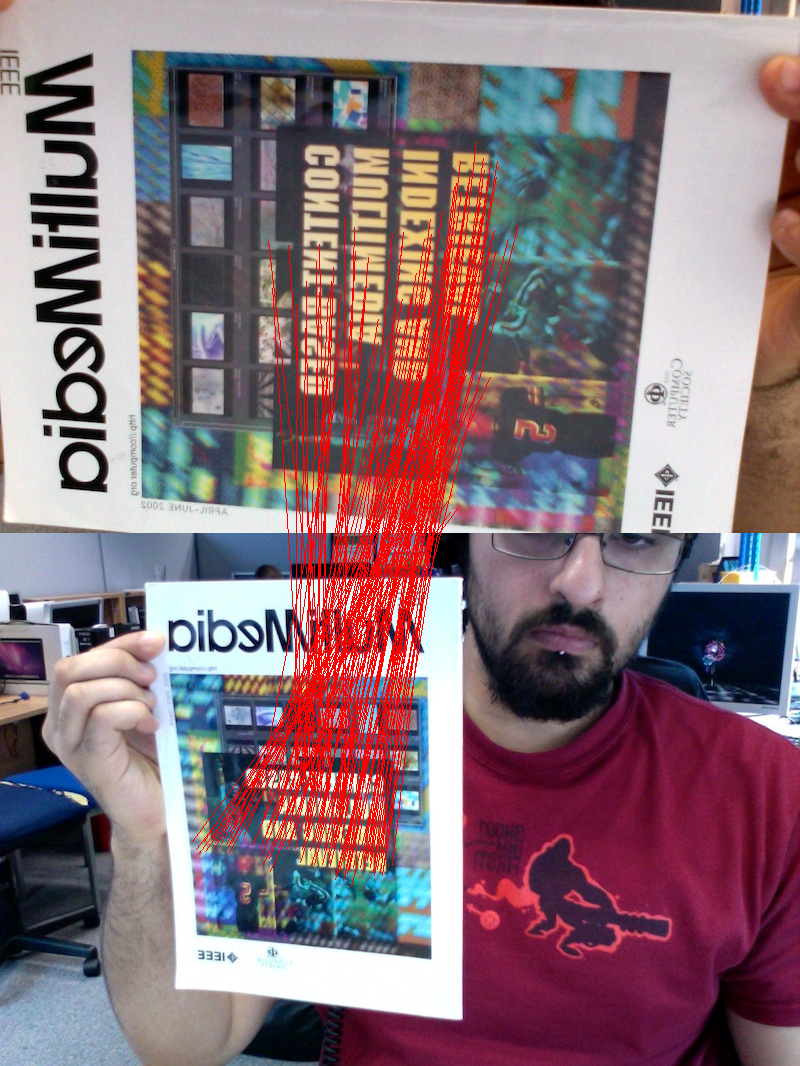
\includegraphics[width=\marginparwidth]{matches-affine.png}}
\begin{lstlisting}[language=java]
DisplayUtilities.display(consistentMatches);
\end{lstlisting}
The \verb+AffineTransformModel+ class models a two-dimensional Affine transform in OpenIMAJ. An interesting 
byproduct of this technique is that the \verb+AffineTransformModel+ contains the best transform matrix 
to go from the query to the target. We can take advantage of this by transforming the bounding box of 
our query with the transform estimated in the \verb+AffineTransformModel+, therefore we can draw a 
polygon around the estimated location of the query within the target:
\begin{lstlisting}[language=java]
target.drawShape(query.getBounds().transform(fittingModel.getTransform().inverse()), 3,RGBColour.BLUE);
DisplayUtilities.display(target); 
\end{lstlisting}
\marginpar{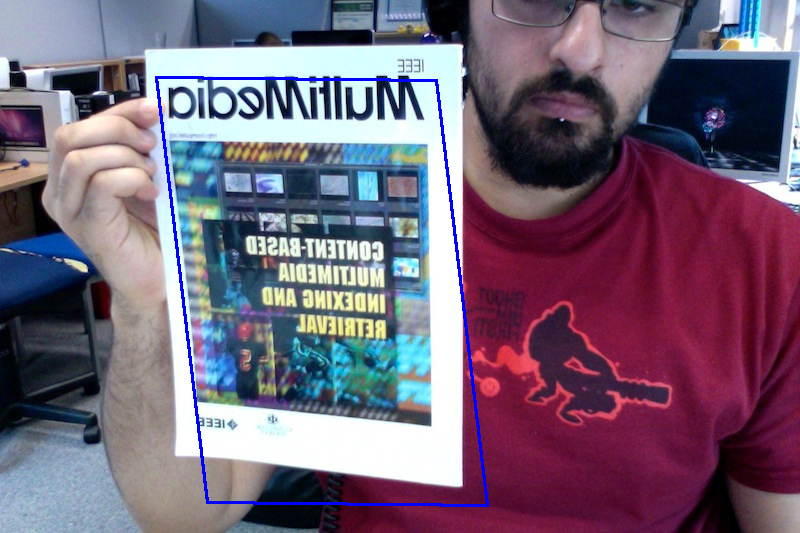
\includegraphics[width=\marginparwidth]{fittedmodel.png}}

\section*{Exercises}
\subsection*{Exercise 1: Different matchers}
Experiment with different matchers; try the \verb+BasicTwoWayMatcher+ for example.

\subsection*{Exercise 2: Different models}
Experiment \marginpar{A \texttt{HomographyModel} models a \textbf{planar Homography} between two planes. Planar
Homographies are more general than Affine transforms and map quadrilaterals to quadrilaterals.}
with different models (such as a \verb+HomographyModel+) in the consistent matcher. 



\end{document}
